\documentclass{article} % Defines the document class, article is commonly used
\usepackage[shortlabels]{enumitem}
\usepackage{amsmath}    % Allows for more advanced math formatting
\usepackage{amssymb}    % Provides additional mathematical symbols
\usepackage{amsthm}     % \qed
\usepackage{graphicx}   % image
\usepackage{float}      % image placement
\usepackage{hyperref}
\hypersetup{
    colorlinks=true,       % false: boxed links; true: colored links
    linkcolor=black,       % color of internal links
}
\usepackage[margin=1.5in]{geometry}
\usepackage{siunitx}

\begin{document}

\title{EEC133 HW4}
\author{Tao Wang}
\date{\today}

\maketitle

\section*{1. The reactance of small loop antennas}
\addcontentsline{toc}{section}{1. The reactance of small loop antennas}
\begin{enumerate}[(a)]
      \item $\boxed{Z_{in} = j Z_0 \tan(kl)}$

            Given the input impedance of a transmission line,
            \[Z_{in} = Z_0 \left(\frac{Z_L + j Z_0 \tan(kl)}{Z_0 + j Z_L \tan(kl)}\right)\]

            Then,

            \[Z_{in}(Z_L = 0) = Z_0 \left(\frac{j Z_0 \tan(kl)}{Z_0}\right) = j Z_0 \tan(kl)\]
      \item $\boxed{\text{Inductor}}$. $\boxed{Z_{in} \approx j Z_0}$
      \item The loop antenna physically look like a shorted transmission line. Therefore, its input impedance is similar to the shorted transmission line from (1), which means it's purely reactive and similar to an inductor.
      \item
            \[\widetilde{A} = j \left(\frac{\mu_0 I A k}{4 \pi r}\right) e^{-jkr} \sin(\theta) \hat{\phi}\]

            \[\widetilde{H} = \frac{1}{\mu_0} \nabla \times \widetilde{A} = j \left(\frac{IAk}{4\pi}\right) \nabla \times \left(\frac{1}{r} e^{-jkr} \sin(\theta) \hat{\phi}\right)\]
            \[= j \left(\frac{IAk}{4\pi}\right)\left(\frac{e^{-jkr}}{r^2}2\cos(\theta)\hat{r} - \frac{\sin(\theta)}{r}(-jk)e^{-jkr}\hat{\theta}\right)\]


            \[\widetilde{E} = \frac{1}{j \omega \epsilon_0} \nabla \times \widetilde{H}\]
            \[= j\left(\frac{IAk}{4\pi r}\right)\left((jk)^2 e^{-jkr} \sin(\theta) \hat{\theta} + \frac{e^{-jkr}}{r^2} 2\sin(\theta)\right)\hat{\phi}\]

            Assume that the $\frac{1}{r^2}$ terms dominate in near field, we have

            \[\boxed{\widetilde{E}_{ff} = \left(\frac{IA}{4 \pi r^3} \sin(\theta)\right) 2\eta_0 e^{-jkr}  \hat{\phi}}\]
            \[\boxed{\widetilde{H}_{ff} = j \left(\frac{IAk}{4\pi r^2} \cos(\theta)\right)2e^{-jkr} \hat{r}}\]

      \item
            \[\vec{S} = \widetilde{E} \times \widetilde{H}^*\]
            \[= \boxed{j\left(\frac{IA}{4\pi r^2}\right)^2 \left(\frac{k }{r}\right) 4\eta_0 \sin(\theta)\cos(\theta) \hat{\theta}}\]
      \item
            \[\widetilde{V} = j X_L \widetilde{I}\]
            \[S = \widetilde{V}\widetilde{I}^*\]
            \[= \boxed{j X_L |\widetilde{I}|^2}\]
      \item Both results are in the form $j (\text{reactance}) (\text{current})^2$. It suggests that the input impedance of a loop antenna is purely reactive.
      \item $\boxed{\vec{S}_{av} = 0}$ because the power is imaginary. The result makes sense because the loop antenna in the near field behaves as a inductor, which stores energy and has imaginary power.
      \item Add a $\boxed{\text{capacitor in parallel}}$ to the inductor because the purely negative reactance will cancel the purely positive reactance.
            \begin{figure}[H]
                  \centering
                  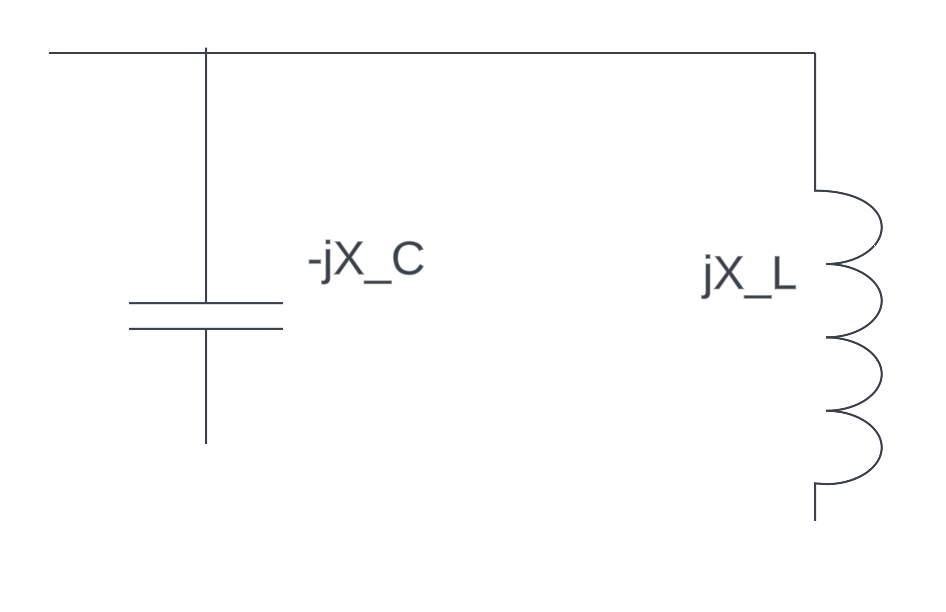
\includegraphics[width=0.5\textwidth]{./image/figure1.png}
                  \caption{A Capacitor in Parallel with a Loop Antenna}
            \end{figure}
\end{enumerate}

\section*{2. The full-wave loop}
\addcontentsline{toc}{section}{3. The full-wave loop}
\begin{enumerate}[(a)]
      \item
            \[\gamma = \frac{Z_L - Z_0}{Z_L + Z_0} = \frac{100 - 50}{150} = \frac{1}{3}\]
            \[|\gamma|^2 = \left(\frac{1}{3}\right)^2 = \boxed{\frac{1}{9}}\]
      \item $\boxed{S = \frac{1 + 1/3}{1-1/3} = \frac{4/3}{2/3} = 2}$. The SWR quantifies the amount of standing wave. The higher the ratio, the higher the amplitude of reflected wave that will form standing waves.
      \item Current Distribution around the loop
            \begin{figure}[H]
                  \centering
                  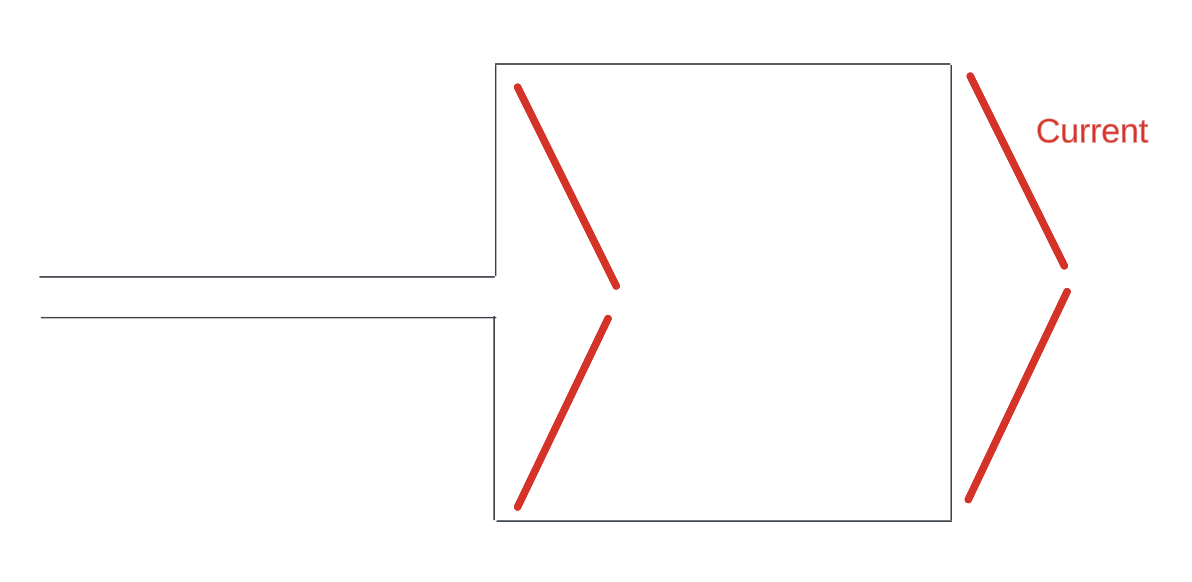
\includegraphics[width=0.5\textwidth]{./image/figure2.png}
                  \caption{Current Distribution}
            \end{figure}
      \item This is not a good approximation because the length of a Hertzian Dipole is $\frac{\lambda}{50}$, but the antenna here is $\frac{\lambda}{4}$ in length.
            \begin{figure}[H]
                  \centering
                  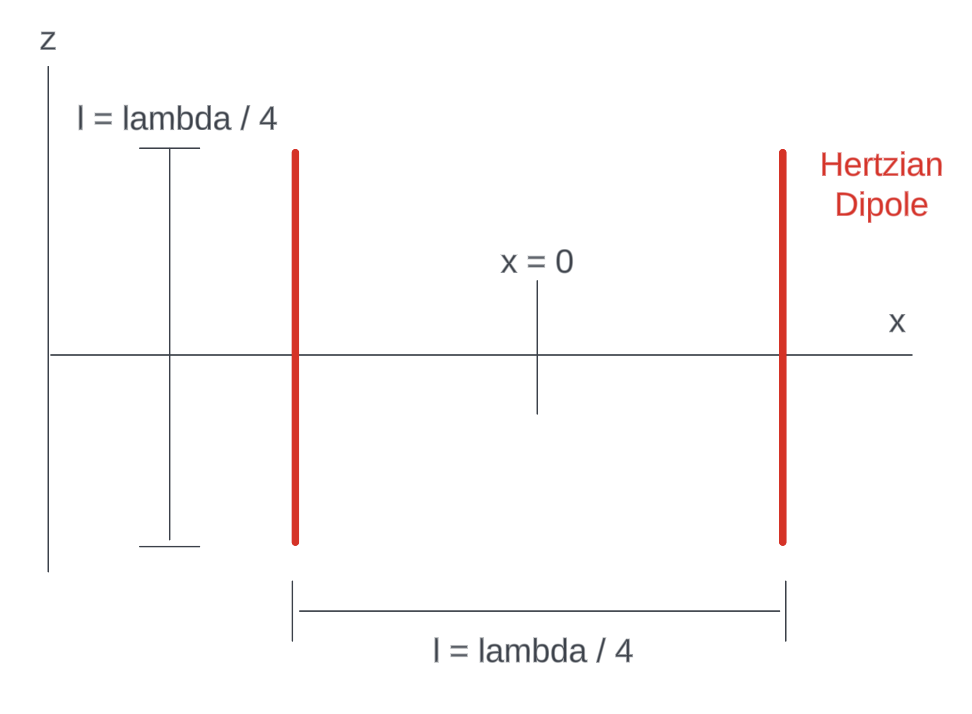
\includegraphics[width=0.5\textwidth]{./image/figure3.png}
                  \caption{Geometry of the Dipole Antennas}
            \end{figure}
      \item
            \[F(\phi) = \frac{1 + 1 + 2 \cos(kl \cos(\phi))}{(1 + 1)^2} = \frac{1}{2} \left(1 + \cos\left(\frac{\pi}{2} \cos(\phi)\right)\right)\]
            \[\boxed{F(x, y) = \frac{1}{2} \left(1 + \cos\left(\frac{\pi}{2} \cos\left(\tan^{-1} \left(\frac{y}{x}\right)\right)\right)\right)}\]
      \item The full-wave loop has a lower directivity because its radiation pattern looks closer to that of the isotropic radiator.
            \begin{figure}[H]
                  \centering
                  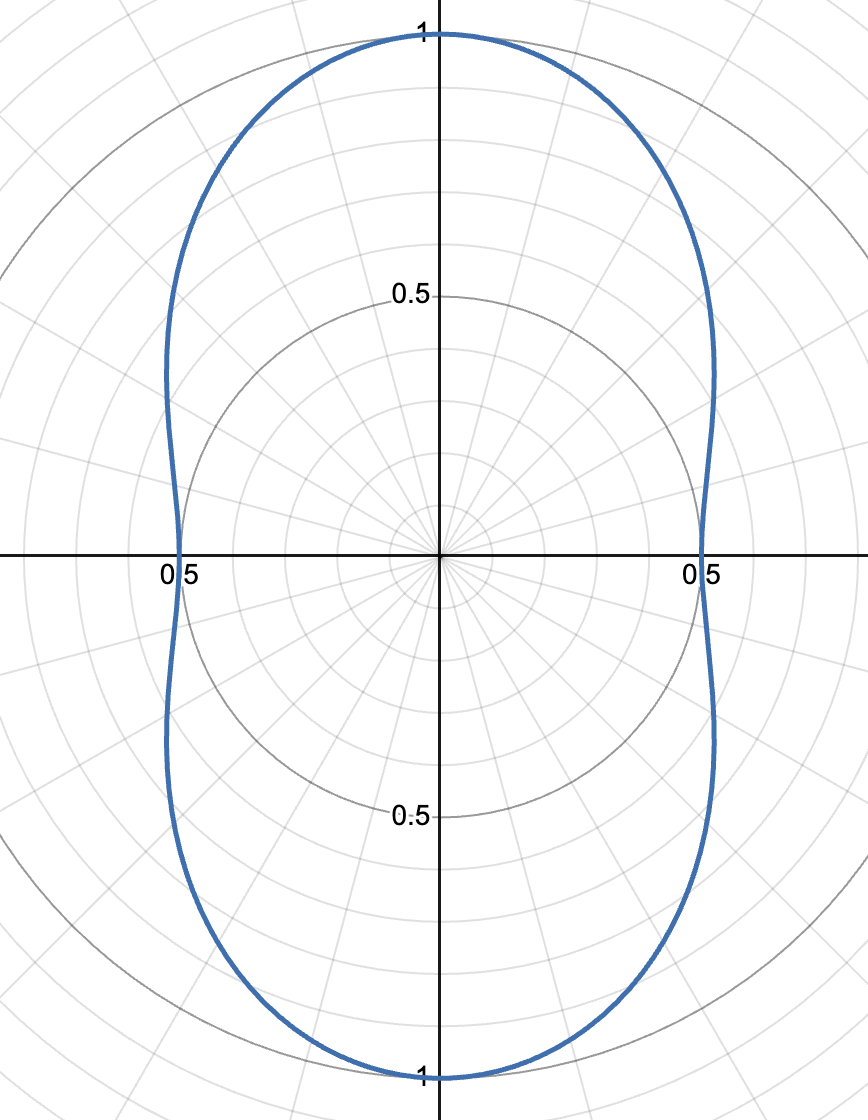
\includegraphics[width=0.5\textwidth]{./image/figure4.png}
                  \caption{Normalized Radiation Intensity with Respect to $\phi$}
            \end{figure}
\end{enumerate}

\end{document}
